%%%%%%%%%%%%%%%%%%%%%%%%%%%%%%%%%%%%%%%%%
% Dossier de conception du projet Picross de l'équipe Craketeam
% 
% Version 2.04
%
% Pensez à éditer le numéro de version (décimal pour les modifications mineures, entier pour les réunions de groupes) et à iniquer vos modifications en dessous.
%
%   Version 2.0(Colas) : Modification de l'entête, des commentaires (traduits ou supprimés), et des packages.
%   Version 2.01(Colas) : Ajout du dictionnaire des données (non exhaustif ni terminé)
%   Version 2.02(Colas) : Modification des noms de mes parties, et complétion de ces dernières.
%   Version 2.03(Colas) : Ajout de la description des Parties Sauvegardée, et modification de la description des scores
%   Version 2.04(Colas) : Ajout des mecanismes de sauvegarde, correction du tableau, et modification des descriptions des différentes données
%   Version 3.00(Colas) : suites aux rectifications vues en groupes quant à la sauvegarde des données, revue des descriptions de chacune des données sauvegardées.
%%%%%%%%%%%%%%%%%%%%%%%%%%%%%%%%%%%%%%%%%

%----------------------------------------------------------------------------------------
%	Packages et documention du document
%----------------------------------------------------------------------------------------

\documentclass[11pt]{article}

\usepackage{fancyhdr} % Required for custom headers
\usepackage{lastpage} % Required to determine the last page for the footer
\usepackage{extramarks} % Required for headers and footers
\usepackage[usenames,dvipsnames]{color} % Required for custom colors
\usepackage{graphicx} % Required to insert images
\usepackage{listings} % Required for insertion of code
\usepackage{courier} % Required for the courier font
\usepackage[utf8]{inputenc}
\usepackage{indentfirst} %Indentation début de paragraphe
\usepackage{float}
\usepackage{colortbl} %Clouleur tableau protoypes de fonctions
\usepackage{tabularx}
\usepackage{placeins}


% Marges
\topmargin=-0.45in
\evensidemargin=0in
\oddsidemargin=0in
\textwidth=6.5in
\textheight=9.0in
\headsep=0.25in

\linespread{1.1} % Line spacing

% Réglages des pieds de page et des en-têtes
\pagestyle{fancy}
\lhead{\hmwkAuthorName} % Top left header
\chead{\hmwkClass\ - \hmwkTitle} % Top center head
\rhead{\firstxmark} % Top right header
\lfoot{\lastxmark} % Bottom left footer
\cfoot{} % Bottom center footer
\rfoot{Page\ \thepage\ sur\ \protect\pageref{LastPage}} % Bottom right footer
\renewcommand\headrulewidth{0.4pt} % Size of the header rule
\renewcommand\footrulewidth{0.4pt} % Size of the footer rule

\setlength\parindent{10pt} % Removes all indentation from paragraphs


\newcommand{\hmwkTitle}{PROJET JEU} % Titre du document
\newcommand{\hmwkDueDate}{Mercredi 5 mars 2014} % Date
\newcommand{\hmwkClass}{DOSSIER DE CONCEPTION } % Type de document
\newcommand{\hmwkClassInstructor}{ } % Teacher/lecturer
\newcommand{\hmwkAuthorName}{Groupe A} % Your name
\newcommand{\hmwkAuthorClasse}{L3 info SPI} % Classe


%----------------------------------------------------------------------------------------
%	Page de Titre
%----------------------------------------------------------------------------------------

\title{
\pagenumbering{roman} \setcounter{page}{0} %La page courante sera numérotée en roman et aura l'indice 0 => Pas de numéro car pas de 0 en roman
\vspace{2in}
\textmd{\textbf{\hmwkClass:\ \hmwkTitle}}\\
\normalsize\vspace{0.1in}\small{\hmwkDueDate}\\
\vspace{0.1in}\large{\textit{\hmwkClassInstructor\ }}
\vspace{3in}
}

\author{\textbf{\hmwkAuthorName}}


\date{\hmwkAuthorClasse} % Insert date here if you want it to appear below your name

%----------------------------------------------------------------------------------------

\begin{document}

\thispagestyle{empty}
\maketitle
\newpage


%----------------------------------------------------------------------------------------
%	Table de matières
%----------------------------------------------------------------------------------------

\thispagestyle{empty}
\pagenumbering{arabic} \setcounter{page}{0} %Le reste du document est numéroté en arabic à partir de la page 1
\renewcommand\contentsname{Sommaire}
\tableofcontents
\newpage


%----------------------------------------------------------------------------------------
%	Présentation générale
%----------------------------------------------------------------------------------------

\newpage

\section{Présentation général}

\subsection{Objectif du document}

Ce document est rédigé dans le cadre du projet de troisième année de licence SPI option informatique de l'Université du
Maine. Le Dossier de Conception vient en complément du Cahier des Charges. Il a pour objectif de monter la modélisation
du système à partir des besoins et contraintes exprimés dans le Cahier des Charges. Il informe également sur les outils
et les normes utilisés pour la conception du produit.

\subsection{Objectif du projet}

L'objectif de ce projet est de concevoir et de développer une application de Picross, ainsi que de rédiger les documents
inhérant à la gestion et la finalisation d'un projet informatique. Les utilisateurs doivent pouvoir, bien évidemment,
jouer, mais il doivent également pouvoir créer des grilles, modifier la taille des grilles, et charger les partie
préalablement sauvegarder. Il doit également être possible de jouer sous son propre profil afin d'avoir accès aux
options les plus poussées de l'application.

\subsection{Documents de références}

Afin de réaliser le présent Dossier de Conception nous nous sommes appuyés sur le Cahier des Charges ainsi que sur les
exemples que nous avons récupérés grâce à un ancien élève de DUT informatique.



%----------------------------------------------------------------------------------------
%	Modélisation du projet
%----------------------------------------------------------------------------------------

\newpage


\section{Modélisation du projet}


\subsection{Les cas d'utilisations}

L'utilisateur de l'application pourra utilisé les différentes fonctionnalités de celle-ci telle que l'édition de grille de jeu, jouer une nouvelle partie, gérer ses parties qui contient la sauvegarde, le chargement, et la suppression d'une partie.
Il pourra aussi quitter l'application à tout moment.

\subsection{Contraintes de conception}

Partie de Kévin
% À ÉDITER!!
\subsection{Le scénario du système}

Partie de Kévin
% À ÉDITER
\subsection{Schéma de navigation}

Le schéma de navigation est composé des différentes fenêtres que compose l'application (les rectangles) ainsi que les possibilités de navigation entre celle-ci (les flèches). Cela permet de visualiser comment on peut passer d'une fenêtre à
une autres à l'interieur de l'application.

%----------------------------------------------------------------------------------------
%	Modélisation de la base de données
%----------------------------------------------------------------------------------------

\newpage

\section{Modélisation de la Sauvegarde des données}

\subsection{Dictionnaire de données}


\begin{tabular}{|p{4cm}|p{3cm}|p{8cm}|} \hline 
    {\bf Nom de l'entité} & {\bf Type } & {\bf Commentaires}\\ \hline \hline
    Grille & Class Ruby Grille & Une collection de case, jointe à un nom et des paramètres ("ALEA20", 20/11/2014)\\ \hline
    Profil & Chaîne de caractère & Le profil joueur, constitué uniquement du nom du profil ("joueur1")\\ \hline
    Scores & Tableau & Un tableau à trois colonnes, comprenant le nom de la grille, le profil et le score\\ \hline
    Parties Sauvegardées & Class Ruby Partie & Partie en cours, sauvegardée avec tous ses paramètres (profil = "", grille ="", temps= --:--, ....) \\ \hline 
\end{tabular}

\subsection{Description des données sauvegardées et de leur stockage}
L'ensemble des données sauvegardées, présentées brièvement ci-dessus, est ici décrite plus en détail.

\begin{description}
    \item [Grille] : les grilles sont les supports du jeu( cf Cahier des Charges 3.1.1). Pour permettre à plusieurs utilisateurs de jouer sur une même grille, il est nécessaire de sauvegarder ces objets. Les grilles sont constituées d'un collection de case, d'un nom, attribué à la création et de divers paramètres, stockés sous formes d'entiers. Elles sont stockés chacune dans un fichier propre, à leur création, qu'elle soit manuelle ou aléatoire. Le dossier des grilles comporte trois fichiers de grilles par défaut.
        % Le stockage peut également se faire autrement, surtout si nous souhaitons proposer aux joueurs de jouer à leurs propres grilles de préférence. Cela peut donc se faire dans un tableau à deux colonnes, l'une indiquant le profil créateur, l'autre contenant la grille. Un tri permettrai de faire ressortir les grilles du profil pour les lui proposer, avec une option "voir toutes les grilles" qui proposerai toutes les grilles. Cependant, on peut envisager que la grille comprend dans ses paramètres le profil du créateur. Le stockage alors n'aurait pas à être modifier, uniquement le comportement lors du chargement du fichier, avec l'enregistrement en mémoire vive d'un tableau pour lequel on récupèrerai le profil du créateur.
    \item [Profil] : Les profils sont les noms que choisissent les utilisateurs(cf Cahier des Charges 3.1.2, qui les définissent dans le jeu, et qui les lient aux grilles créées, aux parties jouées et aux scores. Un profil est principalement constitué d'une chaîne de caractères, choisie par l'utilisateur à la création du profil. Cette chaîne est utilisée à la sérialisation du profil en tant que nom du fichier sur lequel sont sauvegardée les informations du profil. Cette chaîne, de nouveau entrée par l'utilisateur, servira à retrouver et charger son profil
    \item [Scores] : Les scores sont des entiers, dépendant du temps réalisé pour finir la Grille. La donnée à sauvegarder "Scores" est un tableau à trois colonne, comprenant le score lui même, le nom de la grille sur lequel il a été réalisé, et le nom du profil l'ayant réalisé.
        % Peut-être faudra il prévoir plusieurs tableaux, en fonction des différents modes (une colonne indiquant le nombre grille d'affilée en Mode Aventure, etc).
    \item [Parties Sauvegardées] : Elles correspondent à la sérialisation d'une instance de la classe Partie, contenant un certin nombre de paramètres et d'informations, comme la grille utilisée, l'utilisateur, le temps écoulé, etc. Ces paramètres sont conservés sur un fichier lors de la sérialisation. L'utilisateur peut ainsi quitter une partie, fermer le programme, et reprendre cette partie plus tard.
\end{description}

\subsection{Méchanismes de Sauvegarde des Données}
Cette partie détaille l'ensemble des méchanismes de sauvegarde des données précédemment décrites, c'est à dire quand et comment ces données seront sauvegardées ou chargées.

\begin{itemize}
    \item Les Grilles sont sauvegardées après leurs initialisation. Elles sont générées de deux manières : soit aléatoirement, sur demande d'un utilisateur, soit manuellement dans un éditeur. À chaque fois, après avoir été initialisée, la grille est sérialisée via le module YAML et sauvegardée dans un fichier propre au format nom\_createur.nom\_grille. Les grilles sont stockées dans un même dossier, afin de permettre aux utilisateurs de jouer à toutes les grilles, et pas uniquement celles qu'ils sont crées. Lorsqu'un utilisateur souhaite charger une grille, il a le choix entre voir la liste des ses grilles et voir la liste de toutes les grilles(tous créateurs confondus). Une fois qu'il en a choisie une, elle est chargée dans la partie. % Le "_" est un caractère interdit. Il faut le faire précéder par un "\" pour ne pas obtenir d'erreur.
    \item Les Profils sont sauvegardés à leur création. À chaque fois qu'un utilisateur crée un nouveau profil, celui ci est sérialisé et sauvegardé sur un fichier propre via le module YAML. Il est de nouveau sauvegardé à chaque modification. Les utilisateurs entrent leur nom de profil au lancement du jeu, et une recherche dans les dossiers correspondant à chaque profil permet de determiner si le profil en question existe déjà. Une fois le profil trouvé, il est chargé.
    \item Les Scores sont sauvegardés à chaque fin de parties. Ils sont stockés dans un tableau, comme indiqué ci-dessus. À chaque fois qu'un nouveau score est réalisé, il est ajouté au tableau, et le tableau est sérialisé et sauvegardé dans un fichier propre via le module YAML. Le tableau est chargé depuis ce fichier à chaque lancement du jeu via le module YAML.
    \item Les Parties Sauvegardées sont sauvegardées sur demande de l'utilisateur en cours de parties. Elles sont ajoutées à une collection de Parties Sauvegardées, permettant de trier ces Parties, notemment en fonction du Profil joueur, pour proposer à ce dernier de continuer la(les) dernière(s) Partie(s) Sauvegardée(s). À chaque fois qu'une Partie Sauvegardée est ajoutée, la collection est sérialisée et sauvegardée sur un fichier propre via le module YAML. Cette collection est chargée depuis le fichier à chaque lancement du jeu.
\end{itemize}


%----------------------------------------------------------------------------------------
%	IHM
%----------------------------------------------------------------------------------------

\newpage

\section{Interface Homme-Machine}
	\subsection{Introduction}
	Nous allons réaliser l'interface homme-machine concrète correspondant au schéma de navigation ci-dessus. Les principales maquettes à représenter seront donc:
	\begin{itemize}
		\item Accueil
		\item Crédits
		\item Options
		\item Profil
		\item Édition
		\item Jouer
		\item Menu de pause
	\end{itemize}
	
	\subsection{Représentations}
	La première interface apparaissant au lancement de l'application est l'acceil.
	
		\begin{figure}[!ht]
			\centering
			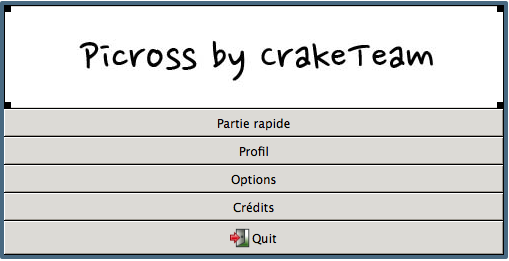
\includegraphics{./IHM/accueil.png}
			\caption{Accueil principal}
		\end{figure}
		
	\FloatBarrier
		
	On peut alors voir les différents choix disponibles.
	Nous allons commencer par les Crédits dans lesquels on peut consulter la liste des développeurs.
	
		\begin{figure}[!ht]
			\centering
			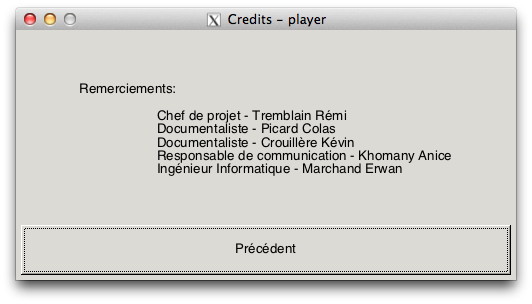
\includegraphics{./IHM/credits.png}
			\caption{Crédit}
		\end{figure}
		
	\FloatBarrier
		
	Nous pouvons ensuite accéder aux options dans lesquels on peut changer la langue par exemple.
	
		\begin{figure}[!ht]
			\centering
			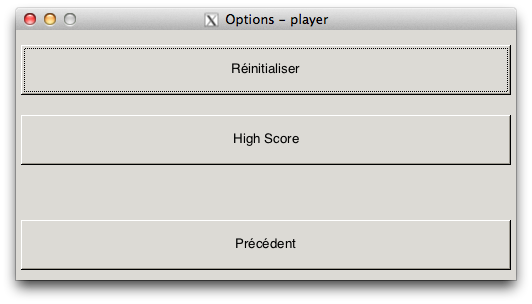
\includegraphics{./IHM/options.png}
			\caption{Options}
		\end{figure}
		
	\FloatBarrier
	
	On peut alors charger ou créer un profil en saisissant son nom.
	
		\begin{figure}[!ht]
			\centering
			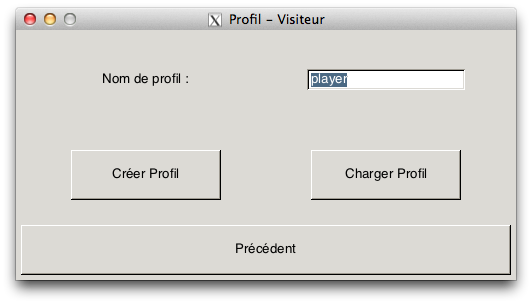
\includegraphics{./IHM/profil.png}
			\caption{profil}
		\end{figure}
	
	\FloatBarrier
		
	Le menu principal change alors pour accueillir la nouvelle option "Édition".
	
		\begin{figure}[!ht]
			\centering
			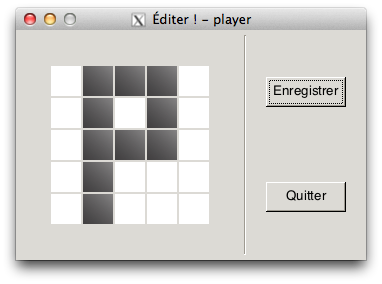
\includegraphics{./IHM/editeur.png}
			\caption{Édition}
		\end{figure}
		
	\FloatBarrier
		
	La principale option reste tout de même le jeu. On doit premièrement choisir entre charger une ancienne partie ou en commencer une nouvelle.
	
		\begin{figure}[!ht]
			\centering
			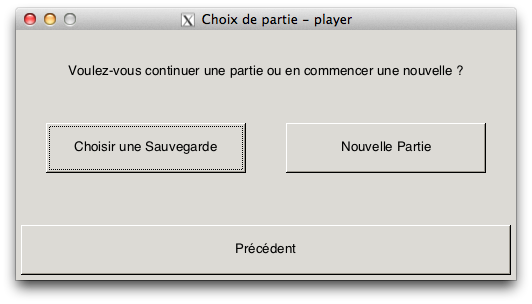
\includegraphics{./IHM/choix_partie.png}
			\caption{Choix d'ancienne ou nouvelle partie}
		\end{figure}
		
	\FloatBarrier
		
	Si on désire charger une ancienne partie, on pourra le faire grâce au menu de sélection de sauvegardes.
	
		\begin{figure}[!ht]
			\centering
			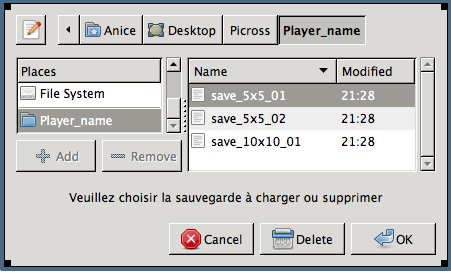
\includegraphics{./IHM/charger_supprimer.png}
			\caption{Charger une partie sauvegardée}
		\end{figure}
	
	\FloatBarrier
	
	En commençant une nouvelle partie, on accède au choix de la taille de grille.
	
		\begin{figure}[!ht]
			\centering
			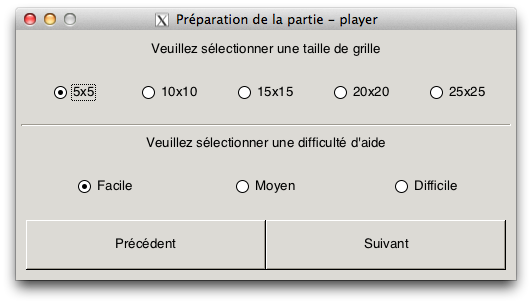
\includegraphics{./IHM/taille.png}
			\caption{Choix de la taille}
		\end{figure}
		
	\FloatBarrier
	
	Une fois la taille sélectionnée, on pourra se lancer dans la partie.
	
		\begin{figure}[!ht]
			\centering
			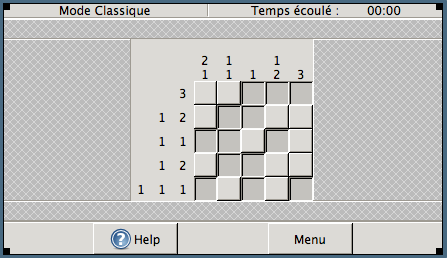
\includegraphics{./IHM/jeu.png}
			\caption{Interface de jeu}
		\end{figure}
		
	\FloatBarrier
	
	Un menu de pause est disponible lors de la partie. Le chronomètre s'arrête et quelque options apparaissent.
	
		\begin{figure}[!ht]
			\centering
			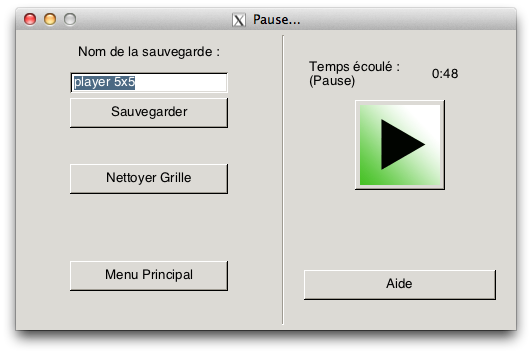
\includegraphics{./IHM/pause.png}
			\caption{Menu de pause}
		\end{figure}
		
	\FloatBarrier
		
	La partie terminée, un menu apparaîtra afin de renouveler l'expérience ou revenir au menu principal.
	
		\begin{figure}[!ht]
			\centering
			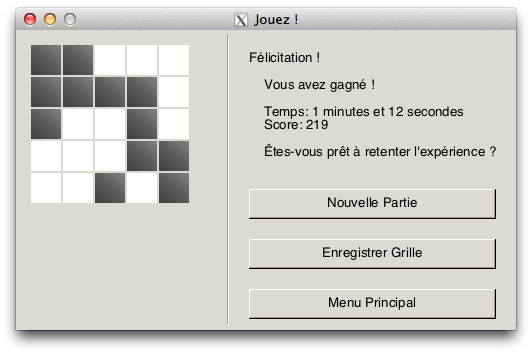
\includegraphics{./IHM/fin_partie.png}
			\caption{Édition}
		\end{figure}
		
	\FloatBarrier
%
%----------------------------------------------------------------------------------------
%	Outils, normes et standards de programmation
%----------------------------------------------------------------------------------------

\newpage

\section{Outils, normes et standards de programmation}

\subsection{Languages utilisées}

Ci dessous nous référençons la liste des différents langages utilisés dans le projet : 

\begin{itemize}
	\item Ruby : Langage de programmation orienté objet, utilisé en version 2.0.0 sur nos machines personnelles, avec une compatibilitée sur les versions antétrieurs,
\end{itemize}

\subsection{Envrionnement et outils de développement}

Le développement sera effectué sur des ordinateurs suffisamment puissants auxquelles nous avons accès à l'Université du Maine, ainsi que sur nos machines personnelles.

\begin{itemize}
		\item Version utilisé de Ruby : 2.0,
		\item GTK : Bibliothèque graphique (The \textbf{G}IMP \textbf{T}ool\textbf{k}it) utilisé avec Ruby.
\end{itemize}

\subsection{Standards de programmation}

Durant le développement, nous respecterons les conventions de codages ci contre : 

\begin{itemize}
	\item Les commentaires doivent être rédigés en français et permettent d'expliquer de façon claire le code.
    \item Le code doit être rédigé de la manière la plus lisible possible (indenté et explicite).
	\item La documentation du code sera faites à l'aide de Ruby doc.
\end{itemize}

\end{document}
